\chapter{Análisis del rendimiento de procesos contenerizados}
\label{ch:03-performance_analysis}

A lo largo del capítulo anterior se han tomado varias decisiones respecto a las
tecnologías que se van a utilizar en el proyecto. El uso de Linux como
plataforma para la ejecución de tareas de tiempo real parte del objetivo
propuesto para este trabajo de analizar las soluciones de tiempo real basadas en
este kernel. Dentro de estas soluciones, aunque las de mayor rendimiento son las
basadas en co-kernels (p. ej., Xenomai y RTAI), hemos optado por usar el parche
\texttt{PREEMPT\_RT}, que aporta las capacidades de tiempo real al propio kernel
de Linux, apoyando nuestra elección en su adherencia a la interfaz estándar del
kernel y la posibilidad de usar las tecnologías de virtualización más conocidas
del mercado. En la sección \ref{sec:02-virtualization} se comprobaba que el
rendimiento de los distintos motores de contenedores es similar, de forma que
decidimos usar Docker para la virtualización de los procesos de tiempo real
debido a ser el motor más maduro y popular.

Una vez definida esta configuración, hemos decidido evaluar su rendimiento
realizando una serie de pruebas. Dado que el rendimiento de Linux con
\texttt{PREEMPT\_RT} es un aspecto que ya ha sido estudiado enormemente en la
bibliografía, nuestro objetivo es más bien analizar el uso de Docker sobre esta
plataforma. Nuestras pruebas se han realizado sobre el dispositivo Raspberry Pi
detallado en la sección \ref{sec:01-tools}. Debido a sus características, la
Raspberry Pi es un dispositivo muy similar a los que nos podríamos encontrar en
una hipotética capa \textit{edge}, de forma que nos sirve para obtener unos
resultados orientativos del rendimiento que se podría obtener en este entorno.

Existen múltiples proyectos comunitarios enfocados a proporcionar utilidades
para la prueba de las características de tiempo real del kernel de Linux, como
es el caso del \textit{Linux Test Project}. Se trata de un conjunto de casos de
prueba para validar la fiabilidad, robustez y estabilidad de Linux, con algunos
orientados a los aspectos de computación en tiempo real. Otro ejemplo lo tenemos
en la suite de pruebas \texttt{rt-tests}, que recoge una serie de programas o
\textit{benchmarks} especialmente centrados en las políticas de planificación de
tiempo real. Hemos decidido usar esta suite en lugar de LTP u otras alternativas
debido a la presencia del programa de prueba \texttt{cyclicdeadline}, que es un
derivado del conocido \texttt{cyclictest}. El objetivo de estos dos programas es
evaluar la latencia en la activación de procesos de tiempo real, es decir, la
diferencia de tiempo entre el momento en el que se debería activar una tarea y
en el que se activa realmente. En \texttt{cyclictest}, esto se hace definiendo
un número determinado de hilos a los que se asignan prioridades diferentes para
ser planificados con la política \texttt{SCHED\_FIFO}. Estos hilos se activan de
forma periódica y se registran las latencias. La principal diferencia que
incorpora \texttt{cyclicdeadline} es el uso de tareas verdaderamente periódicas
planificadas con \texttt{SCHED\_DEADLINE}. Se mide entonces la latencia en la
activación de las tareas para cada período. Como se ha indicado en la sección
\ref{sec:02-real_time}, esta última es la política de planificación elegida para
el sistema que se desea desarrollar, razón por la cuál hemos decidido usar
\texttt{cyclicdeadline} en busca de unos resultados que sean más representativos
del uso real que tendrá el sistema.

Concretamente, se han hecho varias ejecuciones de esta prueba aumentando cada
vez el número de hilos de tiempo real que se debían ejecutar y observar para
poner una carga mayor sobre el procesador y aumentar la complejidad de la
planificación. Para todos los hilos, el límite de tiempo o \textit{deadline} ha
sido de 1000$\mu s$. Estas pruebas se han realizado dos veces: primero,
ejecutando \texttt{cyclicdeadline} de forma «nativa» y, luego, dentro de un
contenedor. La definición de la imagen Docker que contiene la prueba, así como
los pasos seguidos para su ejecución, son explicados detalladamente en el
apéndice \ref{app:C-container_tests}. Los resultados obtenidos son los mostrados
en la tabla \ref{tab:03-cyclicdeadline_latency}. Cabe destacar que
\texttt{cyclicdeadline} solo nos devuelve al final de su ejecución, para cada
uno de los hilos, los valores mínimo, máximo y medio de la latencia. Por ello,
los resultados de la tabla para ejecuciones con más de un hilo muestran
realmente el mínimo de los mínimos de los hilos, el máximo de los máximos y la
media de las medias.

\begin{table}[H]
    \centering
    \begin{tabular}{ | c | c | c | c | c | }
        \hline
                      &                & \textbf{Latencia}         & \textbf{Latencia}         & \textbf{Latencia}        \\
        \textbf{Tipo} & \textbf{Hilos} & \textbf{mínima ($\mu s$)} & \textbf{máxima ($\mu s$)} & \textbf{media ($\mu s$)} \\
        \hline
        Contenedor    & 1              & 1                         & 113                       & 22.0                     \\
        \hline
        Contenedor    & 2              & 1                         & 257                       & 85.0                     \\
        \hline
        Contenedor    & 3              & 1                         & 362                       & 127.33                   \\
        \hline
        Contenedor    & 4              & 1                         & 426                       & 112.0                    \\
        \hline
        Contenedor    & 5              & 1                         & 527                       & 210.20                   \\
        \hline
        Contenedor    & 6              & 1                         & 700                       & 263.0                    \\
        \hline
        Contenedor    & 7              & 1                         & 818                       & 350.29                   \\
        \hline
        Contenedor    & 8              & 1                         & 575                       & 226.5                    \\
        \hline
        Contenedor    & 9              & 1                         & 906                       & 301.78                   \\
        \hline
        Contenedor    & 10             & 1                         & 557                       & 249.6                    \\
        \hline
        Nativo        & 1              & 1                         & 88                        & 17.0                     \\
        \hline
        Nativo        & 2              & 1                         & 267                       & 123.0                    \\
        \hline
        Nativo        & 3              & 1                         & 332                       & 149.0                    \\
        \hline
        Nativo        & 4              & 1                         & 307                       & 122.0                    \\
        \hline
        Nativo        & 5              & 3                         & 448                       & 196.0                    \\
        \hline
        Nativo        & 6              & 1                         & 613                       & 205.67                   \\
        \hline
        Nativo        & 7              & 1                         & 551                       & 225.43                   \\
        \hline
        Nativo        & 8              & 1                         & 729                       & 275.88                   \\
        \hline
        Nativo        & 9              & 1                         & 818                       & 397                      \\
        \hline
        Nativo        & 10             & 1                         & 534                       & 243.2                    \\
        \hline
    \end{tabular}
    \caption{Resultados obtenidos de la ejecución de \texttt{cyclicdeadline}.}
    \label{tab:03-cyclicdeadline_latency}
\end{table}

Lo que queríamos observar con estas pruebas es el impacto que tiene sobre la
latencia el uso de Docker. En la gráfica de la figura
\ref{fig:03-cyclicdeadline_latency}, se muestran los datos de la anterior tabla
de forma que este impacto se hace evidente.  Salvo algunos casos excepcionales,
donde los resultados han sido distintos a la tendencia del conjunto, observamos
como la latencia media se mantiene relativamente similar tanto para la ejecución
nativa como para la contenerizada, mientras que la latencia máxima es la que
experimenta más cambios. No obstante, el impacto no es especialmente notable, de
forma que se puede seguir considerando como una herramienta factible para el
despliegue de procesos de tiempo real, si bien no será recomendable para los que
tengan unas restricciones temporales más pequeñas donde esta latencia sea
demasiado alta.

\begin{figure}
    \centering
    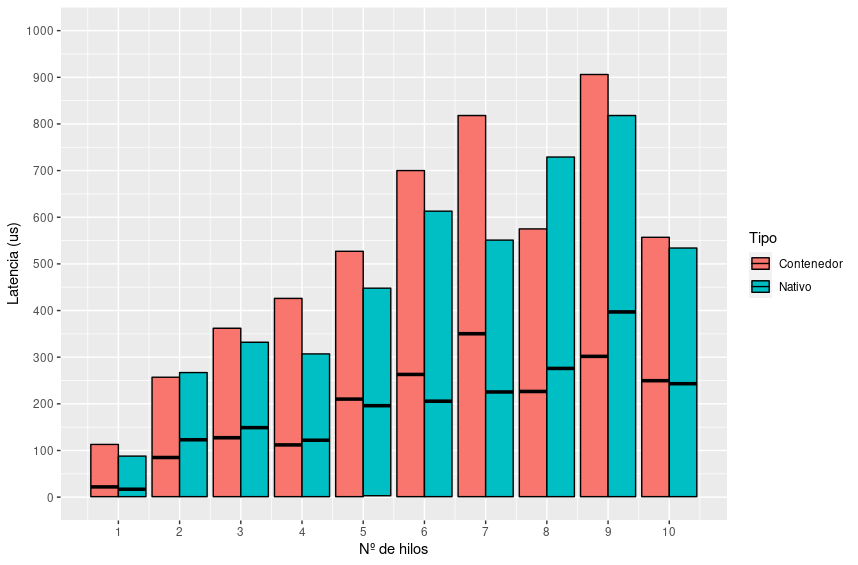
\includegraphics[width=\textwidth]{03-container_analysis/cyclicdeadline-latency.png}
    \caption{Gráfica de intervalos con los rangos de latencia mínima a máxima
        obtenidos de la ejecución de \texttt{cyclicdeadline}. Para cada rango, se
        muestra también su media.}
    \label{fig:03-cyclicdeadline_latency}
\end{figure}

Para caracterizar el incremento en la latencia media aporta el uso de
contenedores, se ha aplicado un modelo de regresión lineal sobre los datos
obtenidos de las pruebas, eliminando los disonantes. El resultado es el que se
muestra en la gráfica de la figura \ref{fig:03-cyclicdeadline_regression}. La
pendiente de la línea obtenida nos indica el aumento que se produce en el
porcentaje de incremento para cada nuevo hilo desplegado, que en este caso es
del 16\%. El valor de $R^{2}$ de este modelo de regresión es 0.96, que, aún no
siendo especialmente alto, sí refleja una correlación evidente entre las
variables.

\begin{figure}
    \centering
    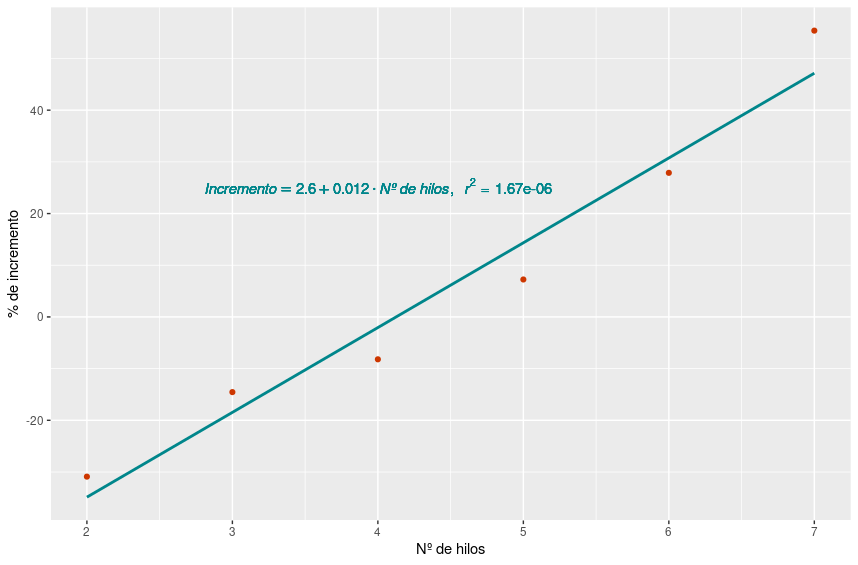
\includegraphics[width=\textwidth]{03-container_analysis/cyclicdeadline-regression.png}
    \caption{Regresión lineal del incremento de latencia según el número de hilos.}
    \label{fig:03-cyclicdeadline_regression}
\end{figure}

Hay que tener en cuenta que la ejecución de \texttt{cyclicdeadline} dentro de un
contenedor se realiza de forma que este programa lanza los hilos de tiempo real
dentro de su mismo contenedor, el cuál ya se encuentra en ejecución. Debido a
esta circunstacia, se decidió realizar una segunda prueba con el objetivo de
analizar la latencia en el lanzamiento de los propios contenedores, dato que es
especialmente interesante en el contexto que se plantea para la herramienta de
orquestación de tareas de tiempo real, dado que estas tareas se deben lanzar en
los nodos desde cero. Para que la ejecución del proceso de prueba no influya en
los resultados, se ejecuta todo este proceso desde un ordenador externo
«maestro». El funcionamiento es el siguiente:

\begin{enumerate}
    \item El maestro lanza un contenedor en la Raspberry Pi mediante SSH.
    \item Cuando el contenedor se lanza, envía un mensaje UDP de vuelta al
          maestro informando de que ha terminado su ejecución.
    \item El maestro obtiene los tiempos de creación e inicio del contenedor
          ejecutando el comando \texttt{docker inspect} mediante SSH.
    \item La latencia se calcula como la diferencia entre ambos tiempos.
    \item El maestro elimina el contenedor de la Raspberry Pi mediante SSH para
          poder lanzarlo de nuevo en la siguiente iteración.
\end{enumerate}

El proceso contenerizado que se despliega en la Raspberry Pi tan solo envía un
mensaje UDP de vuelta al maestro para informar de que ha terminado su despliegue
y ya puede ejecutar \texttt{docker inspect} para obtener las marcas de tiempo.
Se han desarrollado tres implementaciones diferentes de este proceso para
comprobar si el lenguaje de programación usado tiene algún impacto sobre la
latencia. Uno de los lenguajes usados es C, debido a que hoy día se trata de la
\textit{lingua franca} de los lenguajes de programación y es uno de los más
utilizados para la implementación de sistemas empotrados. Para los otros dos,
decidimos optar por Go y Rust. Estos dos lenguajes de programación de sistemas,
gozan de gran popularidad en la actualida entre los desarrolladores, algunos de
los cuales los consideran como alternativas modernas a C. El principal motivo
por el que han sido escogidos sobre otros lenguajes más conocidos como Python
reside en que éste es interpretado, mientras que Go y Rust son compilados. En
lenguajes interpretados es mucho más difícil asegurar que no se van a dar
errores en tiempo de ejecución, lo que es una característica muy importante en
el desarrollo de sistemas empotrados. C++ es otro lenguaje compilado cuyo uso se
consideró, pero al tratarse de una extensión de C y tener un rendimiento
prácticamente idéntico, se decidió por no incluirlo.

Para cada una de las implementaciones, se han realizado 1000 iteraciones de la
prueba, obteniendo los resultados que se muestran en la tabla
\ref{tab:03-container_latency}. En la figura \ref{fig:03-container_latency} se
puede observar una representación gráfica de todas las latencias observadas para
cada iteración.

\begin{table}[H]
    \centering
    \begin{tabular}{ |c|c|c|c|c| }
        \hline
                          & \textbf{Tiempo}        & \textbf{Tiempo}        & \textbf{Tiempo}       & \textbf{Desviación} \\
        \textbf{Lenguaje} & \textbf{mínimo ($ms$)} & \textbf{máximo ($ms$)} & \textbf{medio ($ms$)} & \textbf{típica}     \\
        \hline
        C                 & 1472                   & 2548                   & 1693                  & 165                 \\
        \hline
        Go                & 1445                   & 2718                   & 1693                  & 163                 \\
        \hline
        Rust              & 1478                   & 2378                   & 1701                  & 156                 \\
        \hline
    \end{tabular}
    \caption{Valores observados para la latencia en el lanzamiento de
        contenedores implementados en distintos lenguajes.}
    \label{tab:03-container_latency}
\end{table}

A primera vista, apreciamos que el lenguaje usado para la implementación de los
procesos contenerizados no tiene ningún impacto sobre la latencia en su
lanzamiento. Por otro lado, se trata de valores muy altos, demasiado como para
que podamos considerar el lanzamiento de un contenedor como parte de una tarea
de control estricta. También destaca la gran variación de estas latencias. Todo esto
nos hace pensar que la implementación que tiene Docker de sus tareas de gestión
del ciclo de vida de los contenedores no están preparadas para ser
deterministas, aunque, obviamente, dudamos de que este aspecto fuera considerado
en su diseño.

Sería muy interesante ejecutar estas mismas pruebas usando algún otro motor de
contenedores (p. ej., Podman, Kata, rkt) y así comprobar si, aunque en su
análisis general el rendimiento es similar, en la ejecución de procesos de
tiempo real se observa alguna diferencia. Es más, también se podría probar una
configuración basada en hipervisores para comparar su rendimiento con el de los
contenedores, aunque ya se vió en la sección \ref{sec:02-virtualization} que
éste debería ser parecido \cite{manco_my_2017} \cite{felter_updated_2015}.

\begin{figure}
    \centering
    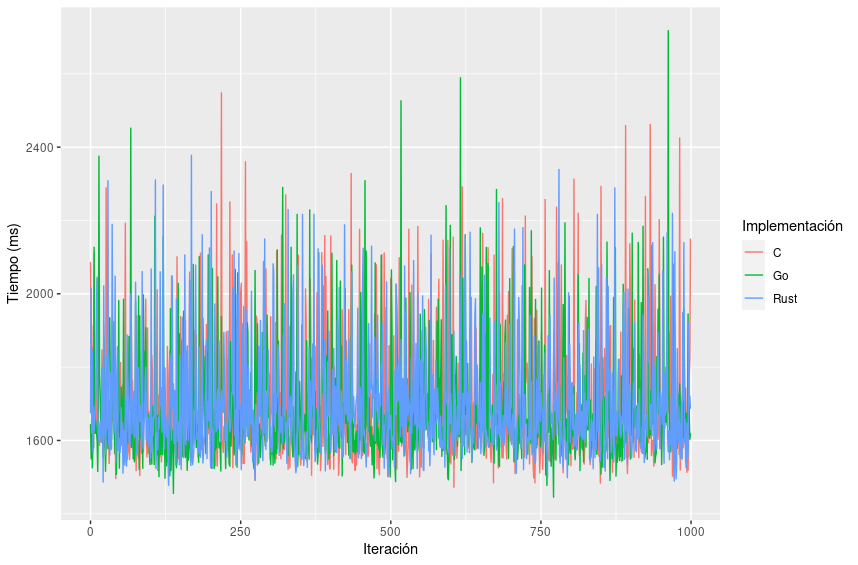
\includegraphics[width=\textwidth]{03-container_analysis/container-latency.png}
    \caption{Gráfico de líneas con las latencias observadas en el lanzamiento de
        contenedores implementados con distintos lenguajes.}
    \label{fig:03-container_latency}
\end{figure}